\chapter{Background}
\label{chp:background} 

This chapter provides a background knowledge of Trusted Execution Environments 
(Section~\ref{sec:trusted-execution-enviroments}), Control-Flow Attacks 
(Section~\ref{sec:control-flow-attacks}), and Anti-Tampering Techniques 
(Section~\ref{sec:anti-tampering-techniques}).
In the final part, we focus on Software Guard eXtension 
(Section~\ref{sec:software-guard-extension}).
These concepts will stem at the base of the following chapters.

\section{Trusted Execution Environments}
\label{sec:trusted-execution-enviroments}

A Trusted Execution Environment (TEE) is a secure area that is contained in the 
main memory (RAM) and is handled by the main CPU~(\cite{Sabt2015TrustedEE}).
A TEE ensures isolation of the code and data against external threats, such as 
the operating system (OS).

The first TEE standard has been defined by OMTP, a forum of mobile 
manufacturers, and the specifications were mainly designed for mobile 
platforms~(\cite{omtp}).
Nowadays, TEEs have evolved into varied scenarios that 
range from mobile platforms to cloud servers~(\cite{schuster2015vc3,sgxtor}).
In the following, we first discuss the two main concepts at the base for this 
thesis: \emph{memory isolation} (Section~\ref{ssec:memory-isolation}) and 
\emph{remote attestation} (Section~\ref{ssec:remote-attestation}).
Then, we describe the common threat model assumptions 
(Section~\ref{ssec:attacker-model}).

\subsection{Memory Isolation}
\label{ssec:memory-isolation}

One of the main property of a TEE is the capability of isolating a portion of 
memory, that is considered trusted, from the rest of the system, that  is 
considered untrusted.
This property allows a TEE to define a parallel environment that can run 
independently by the operation system.
In jargon, the protected portion of memory is called \emph{trusted 
region}, while the outside one is called \emph{untrusted region}.

The implementation of the memory isolation differs by the actual TEE product.
Modern TEE technologies achieve isolation by extending the Memory Management 
Unit (MMU) and the CPU 
cache~(\cite{winter2008trusted,gilmont1999enhancing,rozas2013intel}).
In Section~\ref{sec:software-guard-extension}, we discuss the memory isolation 
of Intel Software Guard eXtension, which is the main technology 
used in this thesis.
                 

\subsection{Remote Attestation}
\label{ssec:remote-attestation}

Remote Attestation (RA) is a challenge response protocol that involves a 
\emph{Prover} and a \emph{Verifier}~(\cite{bajikar2002trusted}), with the 
latter responsible for verifying the current status of the former. 
The \emph{Verifier} sends a challenge to the \emph{Prover} asking to 
measure specific properties. The \emph{Prover}, then, calculates the required 
measurement (\eg a hash of the application loaded) and sends back a report R, 
which contains the measurement M along with a digital fingerprint F, for 
instance, $R = (M,F)$. Finally, the \emph{Verifier} evaluates the report, 
considering its freshness (\ie the report has not been generated through a 
replay attack) and correctness (\ie the \emph{Prover} measurement is valid). It 
is a standard assumption that the \emph{Verifier} is trusted, while the 
\emph{Prover} 
might be compromised. However, the \emph{Prover} is able to generate a correct 
and fresh report due to its trusted anchor (\eg a dedicated hardware module or 
a TEE).
In the following, we describe the two main RA schemes topology: 
\emph{static} RA and \emph{runtime} RA.

\paragraph{Static RA.}
Historically, static Remote Attestation (\emph{static RA}) is the first type of 
RA proposed~(\cite{bajikar2002trusted}).
As the name suggests, \emph{static RAs} measure static properties of a system, 
such as the correct loading of a piece of code in memory through hash functions.
Other technologies, instead, extend their protection and report hardware 
information, for instance, they provide a CPU 
identification~(\cite{anati2013innovative}) or report specific hardware 
configuration~(\cite{sailer2004design}).

\paragraph{Runtime RA.}

%In comparison to \emph{static RA}, the \emph{runtime RA} is relatively new, 
%and 
%today there are no reliable products available on the market since researchers 
%have mainly investigated runtime RA for embedded 
%devices~(\cite{abera2016c,zeitouni2017atrium,aberadiat,dessouky2017fat,Dessouky:2018:LLH:3240765.3240821}).

Runtime Remote Attestation (\emph{runtime RA}) schemes are protocols that 
measure dynamic properties of a system.
For instance, they ensure a piece of code have been executed correctly (\ie 
execution-flow measurement), or they report which modules have been traversed 
by a variable (\ie data-flow measurement).
In the literature, there are many approaches to implement a runtime RA.
For what concerns runtime RA for execution-flow properties, most of them encode 
the complete execution path of a \emph{Prover} in a single 
hash~(\cite{abera2016c,zeitouni2017atrium,dessouky2017fat}); 
some compress it in a simpler representation and rely on a 
policy-based verification schema~(\cite{aberadiat}); 
other ones adopt symbolic execution to verify the control-flow information 
continuously sent by the 
\emph{Prover}~(\cite{Dessouky:2018:LLH:3240765.3240821}).
Runtime RA for data-flow, instead, simply traces the module traversed by 
tainted variables~(\cite{apex,aberadiat}).

All the aforementioned works rely on a trusted anchor (\eg a TEE) to store 
partial results of their protocol (\eg execution-flow information) and for 
protecting crypto materials (\ie algorithms and keys).
Furthermore, they assume the adversary cannot tamper with the trusted anchor.
Finally, \emph{runtime RAs} also assume a \emph{static RA} in place to avoid 
software tampering.

\subsection{Attacker Model}
\label{ssec:attacker-model}

In TEE scenarios, the goal of an adversary is to bypass the TEE protections 
(\ie memory isolation and remote attestation) and tamper with the \emph{trusted 
regions} or alter their behavior.
To achieve this goal, TEsE assume two types of adversaries: \emph{software} and 
\emph{physical}.

\paragraph{Software Attacks.} 
In this case, the adversary works either from a remote location or in the 
\emph{untrusted} memory of the machine (\eg the OS).
In addition, the adversary may control the network medium as in the Dolev-Yao 
model~(\cite{dolev}).
The purpose of the adversary is multifold: she may load a infected software in 
the TEE, alter a \emph{trusted component} already loaded, or use classic 
software exploitation techniques.

The TEE memory isolation prevents an adversary to load compromised software or 
directly modify existing protected ones (Section~\ref{ssec:memory-isolation}).
However, this protection alone does not avoid an adversary to exploit known 
errors to alter the execution of the TEE module trough execution-flow 
attacks.
If the \emph{secure software} suffer of bugs (\eg a memory corruption error), 
the TEE itself cannot prevent an adversary to alters \emph{secure software} 
execution, and finally, the attack happens unobserved.
We discuss execution-flow attacks in Section~\ref{sec:control-flow-attacks}.

\paragraph{Physical Attacks.}
In this case, the adversary has the same goal of the \emph{software 
one} and share the same properties. In addition, the physical adversary have 
access to the machine hardware and can control the hardware components.
Modern TEE technologies alone struggle at defending such attacks, however, it 
is common to assume the adversary requires a non-negligible amount of time to 
carry a physical attck (\eg 10 min - 
\cite{conti2010smallville,conti2008emergent,darpa,ibrahim2017seed,pasta,us-aid}).
Recently, researchers proposed advanced RA schemes to mitigate these 
attacks~\citep{darpa,visintin2019safe,pasta}.

Commonly, denial of service (DoS) attacks are not considered in TEE scenario, 
and the \emph{untrusted software} can avoid invoking the secure module.

\section{Control-Flow Attacks}
\label{sec:control-flow-attacks}

Solely TEE memory isolation and static RA cannot avoid classic exploitation 
techniques.
For instance, a \emph{trusted region} may suffer from a memory corruption 
error that lead an adversary to corrupt a control structure (\ie a return 
address in the stack) and hijack the execution.

To introduce control-flow attacks, we first discuss the concepts of 
control-flow graph (CFG), execution path, and basic-block~(BBL) by using the 
simple program shown in Figure~\ref{fig:problem-setting-code} as a reference 
example. 
The program starts with the acquisition of an input from the user (line $1$). 
This is evaluated (line $2$) in order to redirect the execution towards the 
retrieval of a privileged information (line $3$) or an unprivileged one (line 
$4$). Then, the retrieved information is stored in a variable ($y$), which is 
returned as an output (line $5$), before the program properly concludes its 
execution (line $6$). 

\begin{figure}[t]
	\centering
	\begin{subfigure}[t]{0.45\textwidth}
		\centering
		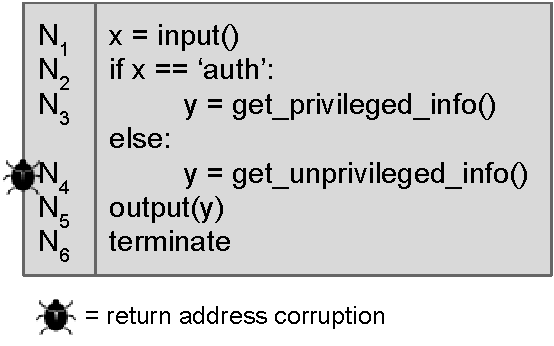
\includegraphics[width=\linewidth]{fig_c4/problem-setting-code.pdf}
		\caption{Pseudo-code of a program under a control-flow attack.}
		\label{fig:problem-setting-code}
	\end{subfigure}
	\hfill
	\begin{subfigure}[t]{0.4\textwidth}
		\centering
		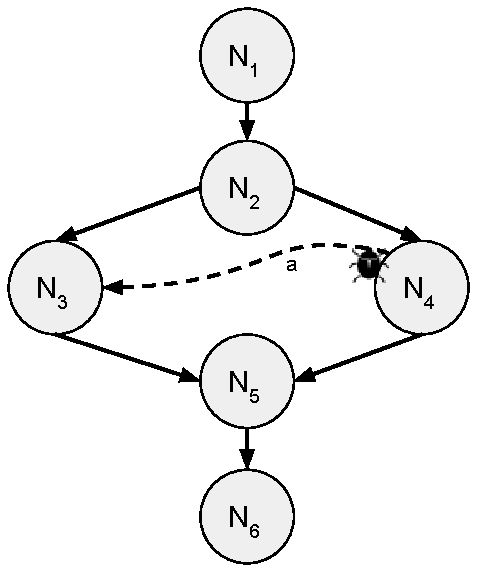
\includegraphics[width=\linewidth]{fig_c4/problem-setting-graph.pdf}
		\caption{Control-flow graph of a program under a control-flow attack.}
		\label{fig:problem-setting-graph}
	\end{subfigure}
	\caption[Example of control-flow attack.]{Illustrative example of a 
	control-flow attack.}
	\label{fig:problem-setting}
\end{figure}

A CFG represents all the paths that a program
may traverse during its execution and it is statically computed. 
On the contrary, an execution path is a single path of the CFG traversed by the 
program at runtime. 
The CFG associated to the program in Figure~\ref{fig:problem-setting-code} is 
depicted in
Figure~\ref{fig:problem-setting-graph} and it encompasses two components: nodes 
and edges. The former are the BBLs of the program, while the latter represent 
the standard flow traversed by the program to move from a BBL towards the next 
one. A BBL is a linear sequence of instructions with a single entry point
(\ie no incoming branches to the set of instructions other than the first), 
and a single exit point (\ie no outgoing branches from the set of instructions 
other than the last). Therefore, a BBL can be considered an atomic unit with 
respect to the control-flow, as it will either be fully executed, or not 
executed at all on a given execution path.
A BBL might end with a control-flow event, which could be one of the following 
in a \texttt{X$86\_64$} architecture: procedure calls (\eg \texttt{call}), 
jumps (\eg \texttt{jmp}), procedure returns (\eg \texttt{ret}), and system 
calls (\eg \texttt{syscall}). 
%Upon certain events (\eg receiving an input), the OS starts a new process.
During its execution, a process traverses several BBLs, which completely define 
the process execution path.

Runtime attacks, and more specifically the control-flow ones, aim at modifying 
the CFG of a program by tampering with its execution path.
Considering Figure~\ref{fig:problem-setting}, we assume that an attacker is 
able to run the program (from the node $N_1$), but that he is not authorized to 
retrieve the privileged information.
However, the attacker can, anyway, violate those controls through a memory 
corruption error performed on the node $N_4$.
As soon as the attacker provides an input to the program and starts its 
execution, he will be redirected to the node $N_4$.
At this point, the attacker can exploit a memory corruption error (\eg a stack 
overflow) to introduce a new edge from $N_4$ to $N_3$ (edge labeled as $a$) and 
retrieve the privileged information.
As a result, the program traverses an unexpected execution path not belonging 
to its original CFG.
Even though several solutions have been proposed to mitigate such attacks (\eg 
ASLR~-~\cite{kil2006address}), attackers still manage to perform 
them~(\cite{van2012memory}). 

This illustrative example about how to manipulate the execution path of a 
program is usually the basic step to perform more sophisticated attacks like
exploiting a vulnerability to take control of a 
process~(\cite{yuan2015hardware}) 
or installing a persistent data-only malware without injecting new code, 
once the control over a process is taken by the 
attacker~(\cite{vogl2014persistent}).

%Runtime RA provides a reliable mechanism which allows the \emph{Verifier} to 
%trace and validate the execution path undertaken by the \emph{Prover}. 

\section{Anti-Tampering Techniques}
\label{sec:anti-tampering-techniques}

We say that a program $P$ is tamper-resistant if $P$ is designed such that an 
attacker would have difficulties to modify $P$'s code.
There are several strategies for achieving this 
goal~(\cite{nagra2009surreptitious}).
In this thesis, we mainly focus on \emph{self-checking}.
These techniques work at bytecode level, and they are structured such that the 
software can read its own bytecode in order to find anomalies and then reacts 
accordingly.
We call \emph{checkers} those sections of the software which check the software 
status, and \emph{responses} those which react to the checkers' requests.

A checker's duties include reading a portion of the software's bytecode and 
verifying whether that code matches specific expectations. That is, the checker 
computes a hash code of the bytecode using a hashing function and compares the 
hash value with a pre-computed value. 
Once a mismatch is found, the software might adopt different reactions, \eg it 
can emit an alarm or restore the un-tampered code. 

To prevent the checkers from being disabled by an attacker, they typically 
spread over the code and/or triggered randomly during the execution.
Checkers, hash functions, and hash values can be prone to attack; therefore, an 
anti-tampering protection must be designed for protecting itself.
This is achievable by using different techniques,
\eg through obfuscation techniques~(\cite{banescu2017tutorial}), or a network 
of checkers (which communicate with each other so that if one checker is 
disabled/tampered, other checkers become aware of the attack).

\section{Software Guard eXtension}
\label{sec:software-guard-extension}

In this section, we introduce the technical details of Software Guard 
eXtension (SGX). We will discuss the memory isolation mechanism 
(Section~\ref{ssec:sgx-core-design}), the attestation details 
(Section~\ref{ssec:sgx-remote-attestation}), the development frameworks 
(Section~\ref{ssec:development-frameworks}), and the main control-flow attacks 
for this technology (Section~\ref{ssec:sgx-control-flow-attacks}).

\subsection{SGX Memory Isolation}
\label{ssec:sgx-core-design}

\begin{figure}[t]
	\centering
	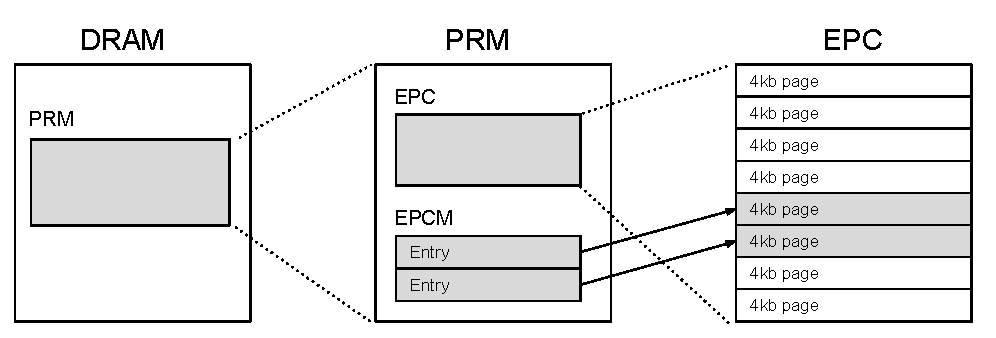
\includegraphics[width=0.8\linewidth]{fig_c7/sgxbackground}
	\caption{Enclave pages architecture in DRAM.}
	\label{fig:sgxbackground}
\end{figure}

The core concept of SGX are \emph{Enclaves}: restricted memory regions 
allocated in DRAM \citep{costan2016intel}.
Figure~\ref{fig:sgxbackground} shows the SGX memory architecture where a subset 
of DRAM, called Processor Reserved Memory
(PRM), is dedicated to the CPU itself (\ie the microcode) and is shielded from
the other system components, such as the operating system, the SMM
code \citep{yao2009system}, and DMA transfers \citep{coke1998implementing}.
The PRM includes an Enclave Page Cache (EPC), which physically contains
the \emph{enclave} pages.
Moreover, since SGX assumes the OS is untrusted, the PRM also contains a 
specific structure, called Enclave Page Cache Map (EPCM), that keeps trace of 
the \emph{enclave} page status.
The EPCM assists the microcode in performing further security controls to block
cross-\emph{enclave} memory access or multiple \emph{enclave} page allocations.

The SGX specifications define four types of EPC pages:
\begin{enumerate}
	\item SGX Enclave Control Structure (SECS) contains the \emph{enclave} 
	metadata.
	The SECS is used by the CPU as a unique \emph{enclave} identifier and is 
	the only page not mapped in user-space, as only the CPU microcode is 
	allowed to read and write it.
	\item The Thread Control Structure (TCS) contains information about a 
	trusted thread running on the \emph{enclave}, pointers to its stack, and 
	other internal status structures \citep{intel-developer-guide}.
	\item State Save Area (SSA) handles exceptions generated from within an 
	\emph{enclave}.
	\item Regular pages (REG) contain code and data.
\end{enumerate}

An \emph{enclave} is bootstrapped by using code running in kernel mode
(\ie a kernel driver) and a set of SGX specific opcodes, that are organizes
as leaf functions under two real instructions: \texttt{ENCLS} (at kernel-space)
and \texttt{ENCLU} (at user-space).
In particular, \texttt{ENCLU} requires a TCS address to identify the thread to
execute.
The kernel handles page allocation and eviction. Any evicted page is encrypted
and versioned by the microcode before being stored in non-volatile storage.
In addition, the microcode performs a double-check to validate the correctness 
of the pages against a cryptographic hash stored in SECS 
to prevent replay attacks from the (untrusted) kernel \citep{rozas2013intel}.

An \emph{enclave} can be bootstrapped in debug mode or in release mode.
The debug mode is used during the development of the \emph{enclave} and permits
external software (\eg debuggers) to access the \emph{enclave} memory
pages through dedicated opcodes (\ie \texttt{EDBGRD} and \texttt{EDBGWR}).
Release mode, instead, enforces all the SGX security features and
does not permit to read the content of an \emph{enclave} from the system.
However, to run an \emph{enclave} in release mode, the \emph{enclave} binary
must be signed with a key issued by Intel to the author.

The process that contains an \emph{enclave} is called \emph{host process}, and
interacts with the \emph{enclave} through dedicated opcodes (\ie
\texttt{ENCLU}).
The reserved part of the virtual address space of the \emph{host process}
designated to its \emph{enclave} is called ELRANGE. The ELRANGE contains
all the \emph{enclave} pages and is defined by a base address and its length.
An \emph{enclave} assumes all the code located inside its ELRANGE to be
trusted, while everything outside is untrusted and possibly under control of an
attacker.

\subsection{SGX Attestation}
\label{ssec:sgx-remote-attestation}

SGX introduces an attestation mechanism \citep{anati2013innovative} that can
establish a secure communication channel between an \emph{enclave} or either 
another \emph{enclave} or a generic software (\eg a process in the 
\emph{untrusted region}).
The attestation can be local (on the same machine) or remote (involving remote 
machines).
In case of remote attestation, the \emph{Prover} is an \emph{enclave}, while 
the \emph{Verifier} can be either another \emph{enclave} or a generic software 
\citep{vill2017sgx}.
The SGX remote attestation guarantees a remote third-party to identify the 
integrity of a local \emph{enclave} and the SGX platform running it.
The SGX RA relies on the isolation offered by the CPU to protect the 
cryptographic keys. 
In particular, the SGX RA guarantees two properties:
\begin{enumerate*}[label=(\roman*)]
	\item the host machine has correctly loaded the \emph{Prover} in memory,
	\item the \emph{Verifier} can check the identity of the 
	\emph{Prover} and the machine (\ie CPU) that is loading it.
\end{enumerate*}
However, the SGX RA does not guarantee \emph{runtime} integrity, for instance, 
an adversary can exploit a memory corruption error while the 
\emph{Verifer} cannot detect the attack.

In SGX machines, this process is based on special privileged enclaves,
called \emph{quoting} and \emph{provisioning} enclaves, that are issued by
Intel.
These enclaves produce a cryptographic proof that validates the microcode
version, the CPU unique keys, and the content of the enclave to
be attested. The result of this cryptographic process is sent to an Intel
attestation server which replies with an asymmetric signature. The signature
can be then sent over the network to the remote third-party to prove the
identity and integrity of the enclave and the platform 
\citep{anati2013innovative}.

\subsection{Development Frameworks}
\label{ssec:development-frameworks}

\begin{figure}[t]
	\centering
	\begin{subfigure}[b]{0.9\linewidth}
		\centering
		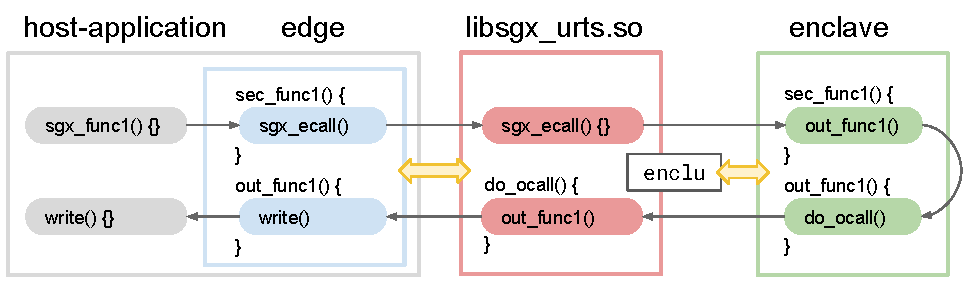
\includegraphics[width=\textwidth]{fig_c7/sgxprogrammingpattern_library.pdf}
		\\[1em]
		\caption{Architecture of an application whose \emph{edge}
			uses \texttt{libsgx\_urts.so} to communicate with the enclave.}
		\label{fig:sgxprogrammingpattern_library}
	\end{subfigure}
%	\\[5mm]
	\hfill
	\begin{subfigure}[b]{0.9\linewidth}
		\centering
		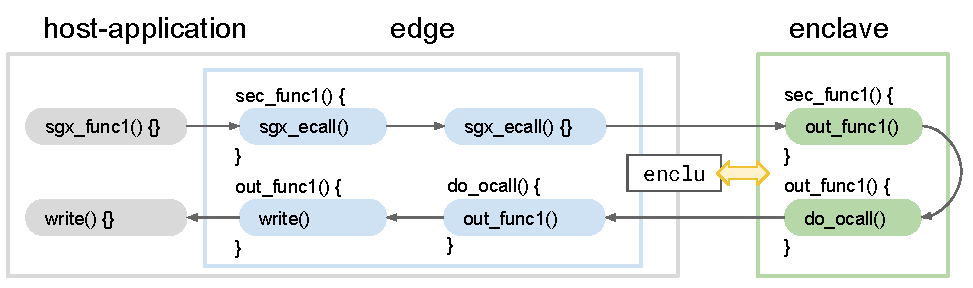
\includegraphics[width=\textwidth]{fig_c7/sgxprogrammingpattern_static.pdf}
		\\[1em]
		\caption{Architecture of an application whose \emph{edge}
			embeds the whole enclave communication logic.}
		\label{fig:sgxprogrammingpattern_static}
	\end{subfigure}
	\caption[Development frameworks' architecture.]{The two main architectures 
	used by an application to communicate with an \emph{enclave}. In both 
	images, the arrow represents the information flow from application to 
	enclave and back.}
	\label{fig:sgxprogrammingpattern}
\end{figure}

A host process that desires to interact with an \emph{enclave} needs to
include specific portions of code that handles the communication with the OS.
In particular, the enclaves mainly relies on two type of functions: 
\emph{secure} (\emph{ecall}) and \emph{outside	functions} (\emph{ocall}). 
The host process uses the former to invoke a piece of code inside an enclave, 
while the enclave triggers the latter to communicate with the operating system 
(\eg to invoke system calls). 
Moreover, both functions invoke an \texttt{ENCLU} opcode directly or indirectly
(\ie through an utility function).
Due to the complexity of this programming pattern, a number
of development frameworks has been proposed to abstract the technical
details and automatically include components in- and outside an
\emph{enclave}.

All the development frameworks share some architecture details.
In particular, part of \emph{secure} and \emph{outside functions} is contained 
in a specific portion of code called \emph{edge}, that is automatically 
generated and statically linked at compilation time.
In our study, we found the \emph{edge} can rely either on external libraries 
(\eg \texttt{libsgx\_urts.so}) to communicate with the enclave, or it embeds
all the communication logic including the \texttt{ENCLU} opcode, as depicted in 
Figure~\ref{fig:sgxprogrammingpattern}.

\subsection{SGX Control-Flow Attacks}
\label{ssec:sgx-control-flow-attacks}

In the following, we described the two main works based on code-reuse 
attacks against SGX: Guard's Dilemma~(\cite{biondo2018guard}) and 
Dark-ROP~(\cite{lee2017hacking}).

\paragraph{Dark-ROP.}
Lee et. al present Dark-ROP~(\cite{lee2017hacking}), a technique to locate 
gadgets in an enclave.
In their scenario, the attacker probes
a victim enclave until triggering an \texttt{AEX}.
From the exception risen, the host can gain information about the location and 
the nature of the gadgets.
Once enough gadgets are collected, the adversary can finally craft a payload 
and bypass the enclave protections.
The success of this technique exploits the fact that neither the enclave 
nor an external observer (\eg the microcode) can backtrack the cause of a 
crash.
In practice, the SGX isolation does not allow inspection either for 
\emph{good} analysis or by adversaries.

\paragraph{Guard's Dilemma.}
Biondo et. al propose a new approach, called \emph{Guard's Dilemma}, that does 
not require probing the enclave~(\cite{biondo2018guard}).
The authors abuse two critical Intel SGX SDK procedures to control the CPU 
registers.
The first one is \texttt{asm\_oret}, that restores the CPU registers after an  
OCALL.
The second one is \texttt{continue\\\_execution}, that is used in the exception
handling.
The authors use the latter to perform a stack pivoting (\ie control the 
\texttt{rsp} register).
\emph{Dilemma} works because the enclave has no mechanism to validate
the integrity of the input of these two functions.